% Drawing 154/02-4 -- folder 154, batch 02, archive page 22 (PDF page 23).
% Transcription: figures, colonne de droite : un faisceau orange sur une droite verte, les deux triangles de part et d'autre hachurés au crayon et marqués $t$, $t'$, le grand triangle $T$ au-dessous, une générisation en pointillé vert ; au-dessous, deux petits faisceaux orange sur une droite verte avec leurs arcs noirs ; plus bas, une petite figure analogue légendée $\operatorname{Pol}^{*}$
% Kind: pencil on a line with specialisation triangles; two small pencils. Method 2 (schematic redraw from the facsimile). Status: ok.
% Notes: Right column: a pencil of orange lines on a green line, the two triangles on either side of the vertex hatched in pencil and marked t', t, the large triangle T below, a green dotted generisation over the vertex; below, two small pencils on a green line with their black arcs, and the legend « Pol*(D) -> Pol(D') ». The « petite figure analogue légendée Pol* » of the transcription is this legend under the two small pencils; no third figure was found.
% Coordinates: 1 unit = 1 mm = 1/100 of the crop width (bbox in page fractions: [0.483, 0.166, 0.701, 0.284]).
% Redrawn by Claude (claude-opus-5-5), issue #73, 2026-11-07; not checked by a human; not compiled (no TeX in the session).
% Rights: reproduces part of the work -- behind RENDER_TRANSCRIPTS, never published by itself.
\documentclass[tikz,border=3pt]{standalone}
\usepackage{amsmath,amssymb}
\usetikzlibrary{patterns,arrows.meta}
\tikzset{Or/.style={orange!90!black}, Ye/.style={yellow!80!orange}, Lg/.style={green!60!black!70}, Dg/.style={green!45!black}, Br/.style={brown!80!black}, Rd/.style={red!85!black}, Bl/.style={blue!70!black}, Gy/.style={black!40}, pencil/.style={black!45}, struck/.style={black!35}, mark/.style={circle,draw,inner sep=1.3pt}, pt/.style={circle,fill,inner sep=0.9pt}, opt/.style={circle,draw,fill=white,inner sep=1.1pt}}
\begin{document}
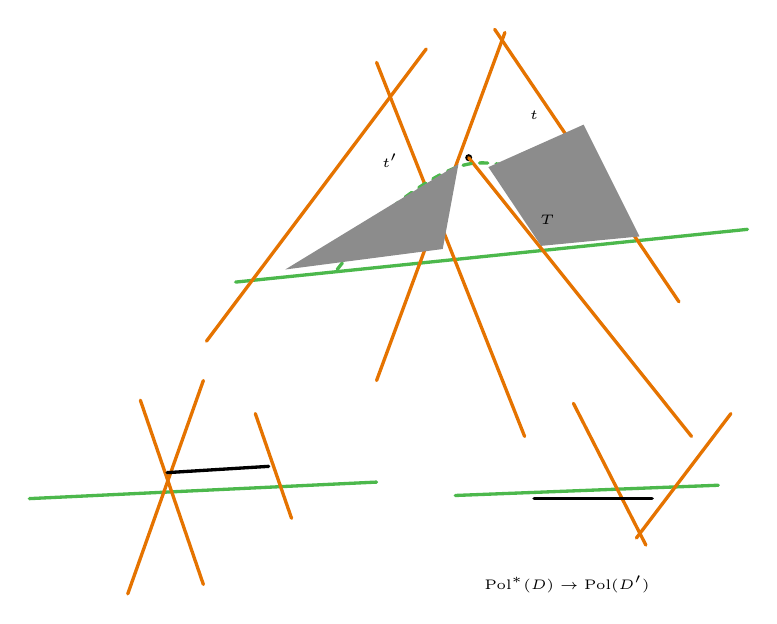
\begin{tikzpicture}[x=1mm,y=1mm,line cap=round,line join=round,font=\scriptsize]
\draw[Lg,very thick] (27.9,-35.4) -- (92.9,-28.7);
\node[pt] at (57.5,-19.6) {};
\draw[Or,very thick] (24.2,-42.9) -- (52.1,-5.8);
\draw[Or,very thick] (45.8,-7.5) -- (64.6,-55);
\draw[Or,very thick] (62.1,-3.7) -- (45.8,-47.9);
\draw[Or,very thick] (60.8,-3.3) -- (84.2,-37.9);
\draw[Or,very thick] (57.5,-19.6) -- (85.8,-55);
\draw[Lg,dashed,very thick] plot[smooth, tension=0.55] coordinates {(40.8,-33.8) (47.9,-25.8) (57.5,-20.4) (67.9,-22.1) (77.9,-27.1)};
\fill[pattern=north east lines,pencil] (34.2,-33.8) -- (56.2,-20.4) -- (54.2,-31.2) -- cycle;
\fill[pattern=north east lines,pencil] (60,-20.8) -- (72.1,-15.4) -- (79.2,-29.6) -- (66.7,-30.8) -- cycle;
\node[inner sep=1pt] at (47.5,-20) {\tiny $t'$};
\node[inner sep=1pt] at (65.8,-14.2) {\tiny $t$};
\node[inner sep=1pt] at (67.5,-27.5) {\tiny $T$};
\draw[Lg,very thick] (1.7,-62.9) -- (45.8,-60.8);
\draw[Or,very thick] (15.8,-50.4) -- (23.8,-73.8);
\draw[Or,very thick] (23.8,-47.9) -- (14.2,-75);
\draw[Or,very thick] (30.4,-52.1) -- (35,-65.4);
\draw[very thick] (19.2,-59.6) -- (32.1,-58.8);
\draw[Lg,very thick] (55.8,-62.5) -- (89.2,-61.2);
\draw[Or,very thick] (70.8,-50.8) -- (80,-68.8);
\draw[Or,very thick] (90.8,-52.1) -- (78.8,-67.9);
\draw[very thick] (65.8,-62.9) -- (80.8,-62.9);
\node[inner sep=1pt] at (70,-73.8) {\tiny $\mathrm{Pol}^{*}(D)\to\mathrm{Pol}(D')$};
\end{tikzpicture}
\end{document}
